\chapter{估算工作量} % Introduction chapter suppressed from the table of contents

这几年大数据很火,很多高科技公司都推相关的工具或者方案,很多软件开发项目经理觉得应该也用数据分析,分析历史数据,准确预估项目工作量、工期。

''但实际上,虽然预测模型已经有超过50年的历史,过千份研究报告,教材/指南,但使用在项目中不多。更多研究发现如果用专家估算可能更准确。``\\
以上是 IEEE杂志 2009 的文章中,JORGENSEN先生的结论。在文章里,JORGENSEN
与 BOEHM 两位专家讨论模型与专家估算法的长短:

%\href{文件:估算专家.png}{300px}

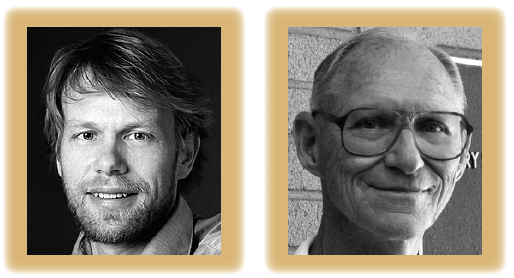
\includegraphics[width=6cm]{估算专家.png}\\

左边:北欧学者 Magne JORGENSEN
过去十多年集中研究软件估算,发现专家估算法虽然很常用,但相关研究却不多\\
右边:Barry BOEHM 81年出版 Software Engineering Economics, 后面又推出
COCOMO 预测模型, 是模型估算的经典人物

\hypertarget{ux4f30ux7b97ux9760ux6a21ux578bux8fd8ux662fux9760ux4e13ux5bb6model-based-vs-expert-based-estimation}{%
\subsection{估算:靠模型,还是靠专家?(Model-based Vs Expert-based
estimation)}\label{ux4f30ux7b97ux9760ux6a21ux578bux8fd8ux662fux9760ux4e13ux5bb6model-based-vs-expert-based-estimation}}

什么是专家估算?最典型的例子,就是WBS估算,我们先把所有的任务,系统地分解出来,召集团队和专家估计工作量(或工期);\\
模型是反过来:利用一些参数模型,如利用功能点数来做其中的一个输入,也包括其他因素,如复杂度、人员能力、平台等。

两种方法的主要区分在于最后估算工作量的步骤:模型(例如COCOMO)通常利用方程式自动从输入估算出结果,如下图:

%\href{文件:估算3.png}{600px}

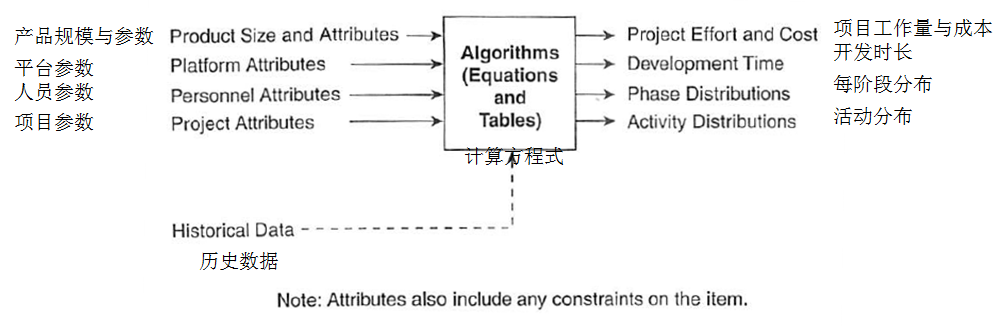
\includegraphics[width=6cm]{估算3.png}\\

或基于国际功能点的ABC模型,依据功能点数,非功能点数,和其他(例如项目管理),ABC
三部分综合估算总工作量(或成本):

%\href{文件:ABC模型.jpg}{600px}

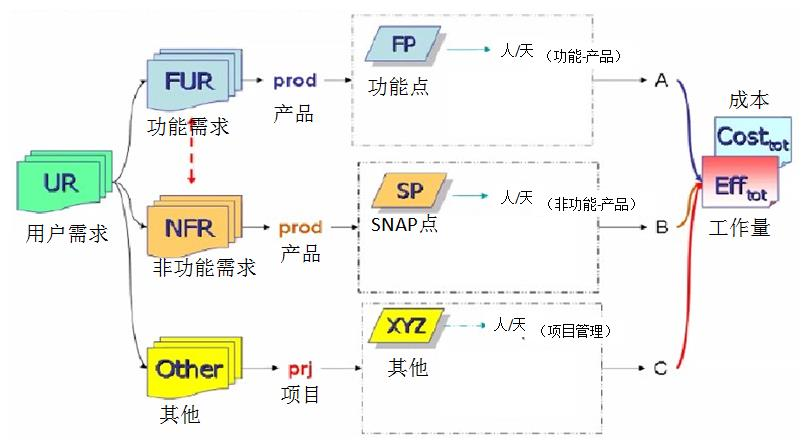
\includegraphics[width=6cm]{ABC模型.jpg}\\

另一方面,专家估算法,例如WBS估算,是以专家主观判断为主(例如,判断活动完成的最可能人天数)。模型估算一般比较客观、可重复性,不像第一种那样主要依赖人的主管判断,但依赖估算专家的能力。

JORGENSEN先生批评模型那派,40多年这么多研究,为什么模型估算还不准确,甚至不如用WBS估算。反过来,BOEHM先生说如果没有模型,整个估算就像个黑盒,无法知道规模、工作量、进度之间的关系,永远靠专家,尤其是在开发的初期,模型特别有用,因为早期需求模糊,无法很准确估算WBS工作量。\\

\framebox{%
\begin{minipage}[t]{0.97\columnwidth}\raggedright
专家估算也有不同的变种,有些纯依赖专家主观判断,有些也会依赖历史数据和检查单,并非仅依赖挑选最佳的专家。有些估算方法,例如,我们一般把扑克牌估算(Planning
Poker)归属于专家估算,但如果最后估算主要依据上一轮冲刺的速度(Velocity)或生产率(productivity),它就更类似模型估算了。

所以虽然模型估算和专家估算看起来有明显差异,但有时候不容易明确区分。下表比较专家与模型估算,总结两种方式的主要区分:

%Screenshotfrom2023-01-0602-48-18.png
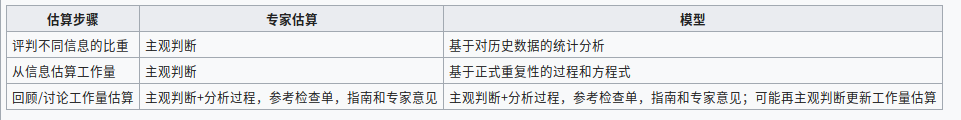
\includegraphics[width=6cm]{Screenshotfrom2023-01-0602-48-18.png}\\

\strut
\end{minipage}}

所以当我们了解为什么不能但靠模型预测,便能理解模型与专家估算,两者各有好处,没有对错,应该两者都要参照。比如模型可以更好地在早期判断,估计整个项目成本,还可以帮我们了解那些因素影响工作量(进度),需要注意。\\

\hypertarget{ux4e3aux4ec0ux4e48ux4f30ux7b97ux5f00ux53d1ux5de5ux4f5cux91cfux5de5ux671fux8fd9ux4e48ux56f0ux96be}{%
\subsection{为什么估算开发工作量/工期这么困难?}\label{ux4e3aux4ec0ux4e48ux4f30ux7b97ux5f00ux53d1ux5de5ux4f5cux91cfux5de5ux671fux8fd9ux4e48ux56f0ux96be}}

你可能会质疑以上的都是大学教授基于学术研究的结论,
实际上数学模型的估算不一定比专家估算差。 我们可以回顾美国SIT的
项目管理估算模拟实验。\\
软件项目管理学生用各种方法估计完成某乐高积木的时长,利用项目数据得出的预算模型的估算准确度还不如戴尔菲法专家估算。(详见附件)\\
由于软件开发很依赖人,主要靠人来做,导致影响生产率的因素很多,如积极性,经验,工具,团队合作等等。用数据挖掘,机器学习,更适合研究一些科学的问题
(物理/化学/生物,如药品的化学成分),相关因素,效用等都好衡量,但是人的因素就没有这么简单。所以过去虽然有几十年的关于工作量的估算模型建立,但准确度一直不太理想。反过来,也不能单靠专家估算,它非常依赖专家的选择,因为人是主观的。虽然主观有可能能帮助做好判断,但也正因为人的主观性,导致估算的偏差。例如,某人做某类软件开发很有经验,她能更准确地估出这类开发的工作量,但如问她能否用一条方程式表达出来,她肯定不知道。\\
所以,如想做好软件开发的工作量估算,首先要理解估算本身的偏差会很大,影响因素很多,也因为无法预测所有(尤其是跟人相关的因素)的影响,个人经验就可以补充估算的不足。

\hypertarget{ux4f30ux7b97ux8f6fux4ef6ux5f00ux53d1ux7684ux56f0ux96be}{%
\subsection{估算软件开发的困难}\label{ux4f30ux7b97ux8f6fux4ef6ux5f00ux53d1ux7684ux56f0ux96be}}

我们有哪个软件开发像玩乐高积木这么直接简单?例如:

\begin{itemize}
\tightlist
\item
  有明确固定的答案;也有明确的步骤,可以照着,按部就班完成
\item
  如果中间过程有错,很容易可立马看出来
\end{itemize}

但软件开发往往是:

\begin{enumerate}
\tightlist
\item
  需求和规范经常有变动(
  大家有哪个项目,需求制定后,到最后开发完成,中间没有变化?)
\item
  软件开发写错一句代码可能影响全盘
\end{enumerate}

因软件开发往往需求不定,所以敏捷大师们反对传统项目估算方式 -
需求(规模)是固定,估算出对应的工期与工作量,并制定整个项目计划与进度表,然后监控,确保项目没有超出计划工期/工时。他们觉得这种以计划驱动的传统管理模式直接影响软件开发团队的生产效率,太多项目因为经理都只是管是否按期完成,是否没有超人时,不考虑软件开发的质量是否给客户价值,反而影响到很多软件项目都被用户诟病。

\framebox{%
\begin{minipage}[t]{0.97\columnwidth}\raggedright
在香港讲敏捷课时,某学员听完敏捷精益的概念后,说她经理要求他她一个三个月的详细工作任务分解,活动详细到五天之内,因为她的经理按计划管理的思路很重。她就很困惑,软件开发变化这么多,怎么可以做出这种详细计划呢?\\其实有点像我们要在一个足球赛还没开始之前,要预先写赛后报告一样没意义,都是猜。\\ 我就回应他说:如果老板有这种思路的话是无法推动敏捷的,其实敏捷有一个很重要的概念,因为需求变化这么大,我们的范围是不固定的,所以基于精益的概念,我们就按有限的时间,制定这个冲刺在两周里面可以完成哪些?做完以后才依据过去的数据进一步策划下一个阶段就更实际了,不是全都靠猜测。这种思路更能让客户尽早看到实际的项目进展,所以敏捷特别重视可以运行测试好的故事,而不是一堆需求文档或者没测试过的代码,因为需求没有给客户看过,还不算是完成,只是一个中间的状态。所以如果经理有这种知道软件开发的特性后,就在那个策划的三角形------时间、成本和规模范围适当取舍,比如,如果我们规定时间为两周,应该可以在那些故事里面挑选最有价值,可以在两周做的故事并完成,展示给客户。就有MVP最小有价值的产物概念,这种就会避免团队为了只追求进度,导致最后做了一大堆没价值的东西,并且很多都没测试好,不能运行。
\strut
\end{minipage}}

我然后跟她说下面这谷歌故事:

\framebox{%
\begin{minipage}[t]{0.97\columnwidth}\raggedright
%\href{文件:Google_Agile_stories_V12esFinal(engCh)v12.png}{600px}\\
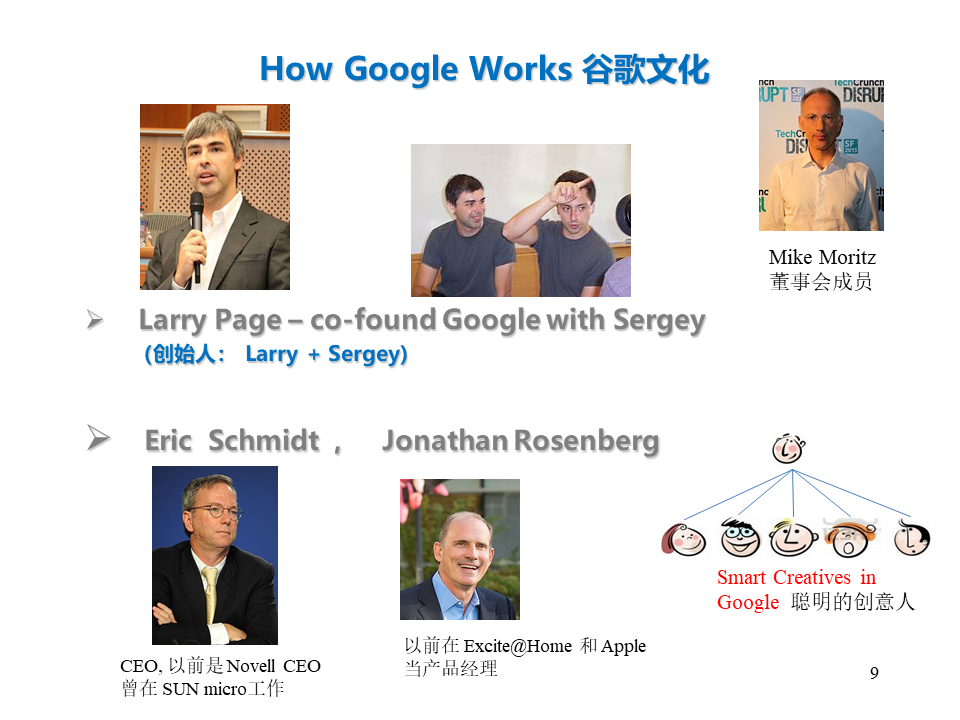
\includegraphics[width=6cm]{Google_Agile_stories_V12esFinal(engCh)v12.png}\\
例如2000年,当时谷歌(Google) 还是很小的公司,但因在搜索引擎有突破,
预计会被微软攻击和收购。

刚进公司的CEO Eric 和 产品经理 Jonathan 便准备了一个详细的两年商业计划。
创始人Larry 看了,便立马问他们俩: ``你们以往有试过超出你们的计划吗?
如果没有,建议还是先跟我们那些工程师聊聊吧。''

后面他们发现Google的工程师都是精英, 无论技术或业务方面的能力都很强,
都有很多创新思路。 了解如果还是按传统的计划驱动反而会
限制了团队的创新能力。\strut
\end{minipage}}

如果团队有能力,应让团队自主创新,传统计划反而会局限了团队发挥,是敏捷开发核心思想。

\begin{itemize}
\tightlist
\item
  因为每次只估算后面迭代(两到四周)的工作量,偏差不会太大
\item
  因为只估算本迭代需求相关工作,减少需求变更的风险
\end{itemize}

因为按范围估算软件开发工作量很困难,
所以只能按有限的资源和时间,识别哪些对客户最重要的功能,
估计能否在项目交付期限内完成。
如果不能,再按功能对客户的价值,选择那些较低的功能可以先不做。

传统项目管理假定规模是固定; 敏捷开发反过来, 时间和资源是固定,
但生产率是按依据团队前面迭代速度的数据。

%\href{文件:微信图片_20230105131327.jpg}{500px}

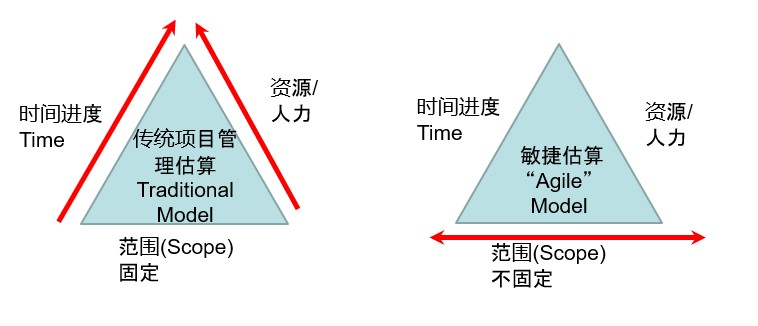
\includegraphics[width=6cm]{微信图片_20230105131327.jpg}\\

这个时间固定,但范围可变的思路,不仅仅适用于软件开发。例如,准备必须月底前将整本书全部交稿,草稿中有不少小错误,如果要全部都修正好,肯定不能按月底期限交付,所以就需要把一些可以删掉的部分删掉,确保书的质量,也把影响降到最低。与软件开发不同,书可以比较轻松删掉一两段,但软件之间的耦合性比较大,可能删掉一行语句整个程序就跑不通,所以更需要在交付前规划好开发的范围,最终才有机会可以按期交付。

敏捷是依据精益MVP概念,时间(资源)固定,范围可变,如果估计不能在交付期限前完成所有客户需求,便要尽早跟客户协商,选择哪些功能放在这次交付之内,哪些放在后面,希望有限的时间和资源条件下,给客户提供最高价值。

很多敏捷团队会用以下方式逐步做估算:\\
先把所有客户的需求写成故事卡片,作为整个项目的交付物(Backlog),然后按每次迭代(例如从第一次迭代):

\begin{itemize}
\tightlist
\item
  先挑选最重要的故事,放在本次迭代,估计相关的故事点,故事点是一个简单的规模概念,团队按照类似的模块的工作量,估计每故事的故事点数(例如,可以用扑克牌举牌方式多轮估算,最终得出一个团队都赞同的故事点数)
\item
  按本迭代可允许的人天数估计本迭代可以完成多少个故事点
\item
  然后每次迭代结束后记录完成多少故事点,形成燃烧图(burndown
  chart),看功能点的降低速度来预估整个项目最终完成的时间,需要多少个迭代。从燃烧图,故事点减少的速度计算项目速度(velocity)。
\end{itemize}

\begin{description}
\item[]
\begin{description}
\tightlist
\item[]
+ + +
\end{description}
\end{description}

有些敏捷大师甚至反对估算(NoEstimate),觉得估算只是凭个人拍脑袋、凭经验,没有依据,反而导致团队只关心进度不能延误,影响开发员,使得开发人员反而不能专心专业地做好软件开发。\\
NoEstimate反对使用故事点估算,故事点按个人经验来估算,不同人的理解不一样,可能导致差异很大。同样,他们也反对敏捷Velocity速度的概念,觉得只是另一个形式的传统策划思维,也会导致团队只是关注一个冲刺迭代交付了多少个故事点,反而忽视了交付的软件是否对确实客户有价值。\\
但他们也理解到团队还是要可以预估可否在客户定的期限件内交付,或者交付多少,因为这是客户关注的。他们建议直接把backlog里要交付的所有需求,细分成小故事,每个故事最好是一人天左右。这样就很简单,可以按完成故事的速度,更客观地预计客户要最后交付的日期(例如,十周后),可以完成多少故事。\\
例如,共要求300个故事,按团队速度,十周后只能总共完成200,就要提前按优先级、重要性跟客户协商,挑选哪些在这个期间前交付,那些放到下一次再做。(前提是:团队必须已经做了一些开发,知道每次两种迭代大概可以完成多少故事。)

\hypertarget{ux603bux7ed3}{%
\subsubsection{总结}\label{ux603bux7ed3}}

选择那种方法估算软件开发工作量,跟选择最合适的项目生命周期方法类似,取决于项目的特性和团队的能力。
如果需求很明确和固定,可没有客户代表在每个迭代(2-4周)确认,例如,政府投标定制开发项目,就不一定选择精益MVP思路的敏捷估算方法,而应依据范围(scope)和规模(size),估算工期与工作量,除了使用WBS分解从下而上靠专家/团队估算工作量与工期外,也要利用规模(功能点数),利用基于历史数据的估算模型从上而下估算。(千万不用以为那种估算最准确,其实都不准,但综合考虑可以减少偏差)

如果需求很可能会变,客户参与,团队能力强的产品性开发项目,时间/资源固定,范围可变的精益敏捷
思路就更能为干系人创做价值。如果可以把范围细分到很小的估算(每故事
\textasciitilde{}1人天),可以依据以往历史速度,估算要完成所有需求一共要多少次迭代(或周);但如果项目复杂,之间相互依赖,有些模块要多人合作,难以细分,就难以用前面的简单线性估算,须要团队估算工作量,但不应只依赖从下而上按任务估计工作量,也要参考规模大小,利用估算模型从上而下估算,然后综合考虑。

%\href{文件:敏捷非敏捷1.jpg}{400px‎}

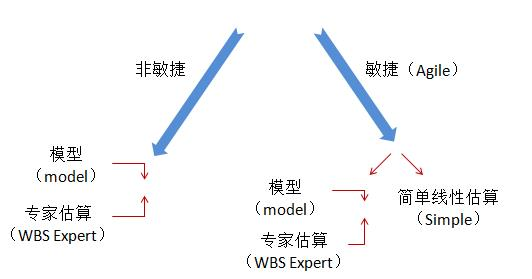
\includegraphics[width=6cm]{敏捷非敏捷1.jpg}\\

\hypertarget{ux9644ux4ef6}{%
\section{附件}\label{ux9644ux4ef6}}

\hypertarget{ux4f30ux7b97ux780cux4e50ux9ad8ux79efux6728ux65f6ux957f---2015ux5e74ux5b66ux751fux5b9eux9a8cux6570ux636e}{%
\subsection{估算砌乐高积木时长 -
2015年学生实验数据}\label{ux4f30ux7b97ux780cux4e50ux9ad8ux79efux6728ux65f6ux957f---2015ux5e74ux5b66ux751fux5b9eux9a8cux6570ux636e}}

2015年,17位有工作经验的兼读学生
参加SIT的软件估算与度量课程(一个学期,共13节课)。
为了让学员亲身感受软件估算的困难,
老师要求学员用以下各种方式估算要完成乐高"Sopwith
Camel"积木(详见下图)的时长:

%\href{文件:Lego1.jpg}{300px}

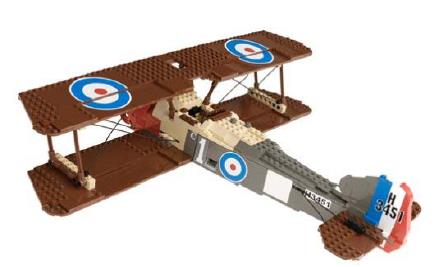
\includegraphics[width=6cm]{Lego1.jpg}\\

\begin{enumerate}
\tightlist
\item
  每位学员独自做估算 (I)
\item
  使用戴尔菲法(Wideband Delphi),多轮后更新(个人)估算 (II)
\item
  分成3组,每组也使用戴尔菲法,制定本组的(团队)估算 (II(团队))
\item
  依据实验数据(注2)调整、更新(个人)估算 (III)
\item
  团队也依据实验数据调整、更新(团队)估算(III(团队))
\item
  完成以上4、5步后,立马告知会选那位学员实际做LEGO积木(注3),让个人调整、更新(个人)估算
  (IV)
\item
  也让团队调整、更新(团队)估算 (IV(团队))
\end{enumerate}

\framebox{%
\begin{minipage}[t]{0.97\columnwidth}\raggedright
注1:

\begin{itemize}
\tightlist
\item
  之前在课程里,已正式学过戴尔菲法
\item
  加上规模,复杂度等对工作量、生产率的影响
\end{itemize}

注2:
让学员自己做乐高实验(因有些学员可能从未玩过乐高积木),提供4对同样的积木:

\begin{itemize}
\tightlist
\item
  Big Ben(下面有完成后的照片)
\item
  Leaning Tower of Pisa
\item
  Eiffel Tower
\item
  General Grievous Wheel Bike
\end{itemize}

%\href{文件:Lego_2.png}{300px}

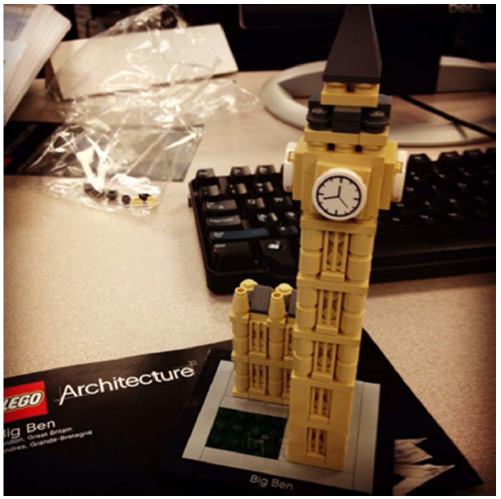
\includegraphics[width=6cm]{Lego_2.png}\\

\begin{itemize}
\tightlist
\item
  每学员记录实际完成的时长,把所有数据汇总并公开给所有人
\item
  之前在课程里,已正式学过预测模型和数据统计基础,如何利用以往数据,建立模型(附件里有如何建模的介绍)
\end{itemize}

注3:

\begin{itemize}
\tightlist
\item
  大家都有这位学员之前乐高实验所需时长的数据
\end{itemize}\strut
\end{minipage}}

\hypertarget{ux5b9eux9a8cux7ed3ux679cux4e0eux8ba8ux8bba}{%
\subsubsection{实验结果与讨论}\label{ux5b9eux9a8cux7ed3ux679cux4e0eux8ba8ux8bba}}

%\href{文件:Lego3.jpg}{600px}

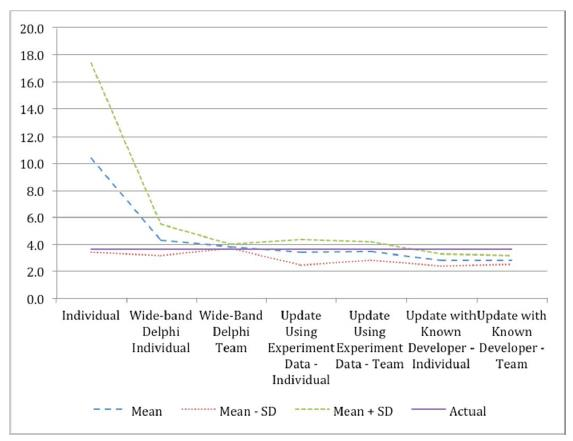
\includegraphics[width=6cm]{Lego3.jpg}\\

\begin{itemize}
\tightlist
\item
  那学员用了213分钟(差不多3.55个小时)完成,他自述困难主要在于颜色都很类似,很多时候找不到合适的积木。(跟其他体验组比较,其他2-3
  组都差不多在210 - 220分钟范围之内完成)
\item
  戴尔非法显著减少了个人估算的偏差,用戴尔菲的团队估算其实是最接近实际的,估得最好的,偏差不超过15分钟。开始时,尤其个人都会多估,但后面数据越来越多,反而开始有点偏低了
\item
  可能导致后面估算偏低的原因:之前实验用的4组积木都是建筑物,复杂度与颜色搭配都较简单
\end{itemize}

\hypertarget{ux7ecfux9a8cux6559ux8bad}{%
\subsubsection{经验教训}\label{ux7ecfux9a8cux6559ux8bad}}

\begin{enumerate}
\tightlist
\item
  学生经过这个过程可以从实验亲身感受到估算的局限,没有想象这么准确,太多因素影响,也很难建立一个预测模型,比如偏差可能到了0.3以上
\item
  从这个过程里面也让他们感受到主观判断的重要性,不要以为仅仅客观用一些数据、用数学方程式就可以准确估出正确的答案
\item
  也了解复杂度和人对生产力的影响,比如积极性跟经验都是很重要的因素。例如,有一个学生经验很少,但竞争力和积极性非常高,所以有好的成绩。有两个团队也是完成同一套??模型,发现本来自己判断为高经验的团队反而比中经验的团队花多一倍时间,最慢的团队是一个两人团队,因为基本没有经验,所以就很小心,一步一步去做,尽量少减少错误,导致用的时间最长。
\item
  团队规模大小也有影响,团队人数越多其实是对整个生产力有负面影响,人数少反而会好一些。(其它关于软件开发的研究也有类似的发现)
\end{enumerate}

很多人以为软件项目估算与其他项目(如土木)类似。以上实验,虽然不是真正做软件开发,学生自己做估算,从亲身体验学习,
更好了解软件项目估算的常见误解:

\begin{enumerate}
\tightlist
\item
  以为软件估算可以精确到正负几个百分点
\item
  以为在项目时间不够的时候,增加人员对项目的进度会有帮助
\item
  以为团队人越多,工期就按比例缩短,像建筑工程一样
\item
  以为估算是可以单靠一些预测模型简单地估出一个数值。
\end{enumerate}

学生都没有软件项目的经验,我们也不可能在上课的时候做软件项目,于是用乐高积木,让他们做估算,比如我们让他们依据一个结果图,估算要多少人时来完成积木,也要看人的乐高经验,首先第一步是他们单独做估算。我们在课程中用了Wideband
Delphi 估算法,每个人多轮估算。找人确实来建乐高,看看实际用了多少时间。
然后我们在课程中加了一些估算模型,用一些历史数据给他们进行参考,下面就是我们的一些发现:很多人在没有经验的时候都会高估,用了Wideband
Delphi 的方式会确实比较准确。
后面有了实际数据,要求学生利用软件项目估算模型方式来估,他们就发现这不容易,很多时候,有学生直接改用简单方程式做估算。
学生自己动手来估算,才会有感觉,真正了解软件估算的各种困难。\\
%Screenshotfrom2023-01-0602-54-00.png
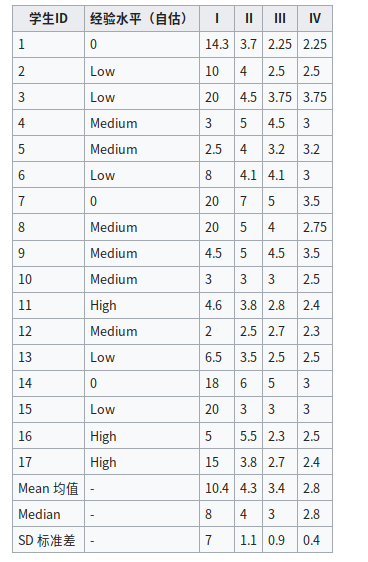
\includegraphics[width=6cm]{Screenshotfrom2023-01-0602-54-00.png}\\

注:上面 I,II,III,IV 与 下面 II,III,IV
的定义,对应那种场景,已经在上面本文里说明。

%Screenshotfrom2023-01-0602-54-26.png
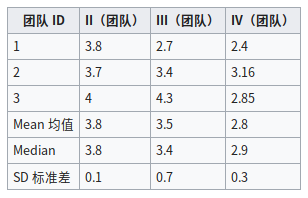
\includegraphics[width=6cm]{Screenshotfrom2023-01-0602-54-26.png}\\


%Screenshotfrom2023-01-0602-55-33.png
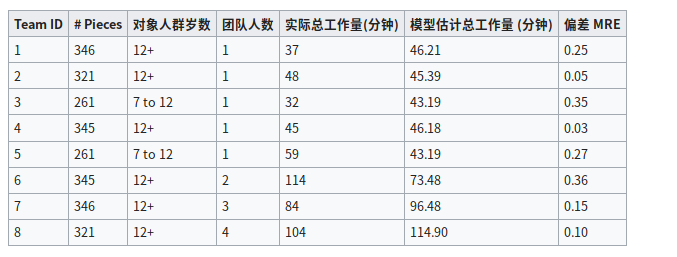
\includegraphics[width=6cm]{Screenshotfrom2023-01-0602-55-33.png}\\
注:偏差 MRE(Magnitude of Relative Error) = \textbar{} (实际 - 估算)
\textbar{} / 实际

\hypertarget{references}{%
\section{References}\label{references}}

1. JORGENSEN, Magne . B. BOEHM: "Software Development Effort Estimation:
Formal Models or Expert Judgment? " , IEEE SOFTWARE, March/April 2009\\
2. LAIRD, Linda, Y. YANG: "Engaging Software Estimation Education using
LEGOs: A Case Study" 2016 IEEE/ACM International Conference on Software
Engineering Companion\\
3. DUARTE,Vasco: \emph{NO ESTIMATES: How to Measure Project Progress
without Estimating}\\


